%\subsection{Preliminary considerations}


\subsection{Intuition and high-level overview}
Let us consider an initial system of multivariate polynomials in $n$ variables, denoted as $x_1, \dots, x_n$, defined over a finite field $\Fq$. 
% Let $d_i$ denote the maximum degree of the polynomials with respect to the target variable $x_i$. 

The core idea of the algorithm relies on a variable elimination strategy. We begin by reinterpreting the polynomial system as a collection of polynomials in the ring $\Fq[x_2, \dots, x_n][x_1]$. In this representation, the system is treated as a set of univariate polynomials in $x_1$, where the coefficients are themselves multivariate polynomials in the remaining variables, specifically in $\Fq[x_2, \dots, x_n]$.

Next, we construct the coefficient matrix of this univariate representation and reduce it to its Row Echelon Form (REF). Through this reduction, the final non-zero block of the matrix yields a linear relation with respect to $x_1$, which takes the form:
\begin{equation*}
    f_1(x_2, \dots, x_n)\cdot x_1 + g_1(x_2, \dots, x_n) = 0
    \label{eq:linear_relation_1}
\end{equation*}

While we cannot generally assume that $g_1$ is divisible by $f_1$, this structural relation provides a crucial substitution mechanism. Returning to the original system, we multiply the equations by an appropriate power of $f_1(x_2, \dots, x_n)$. This homogenization allows us to substitute every occurrence of the term $(f_1(x_2, \dots, x_n)x_1)^k$ with $(-g_1(x_2, \dots, x_n))^k$. This substitution systematically eliminates the variable $x_1$, reducing the dimension of the polynomial system by one.

Such elimination procedure is applied iteratively. Specifically, at any given step $i$ (for $i = 1, \dots, n-1$), the active system is defined over the polynomial ring $\Fq[x_i, \dots, x_n]$. We rewrite this system by treating it as a collection of univariate polynomials in $x_i$, with coefficients belonging to the ring of the remaining variables, namely $\Fq[x_{i+1}, \dots, x_n][x_i]$. 

By constructing the coefficient matrix for this representation and reducing it to REF, we isolate a linear relation for the variable $x_i$, which takes the form:
\begin{equation}
    f_i(x_{i+1}, \dots, x_n)\cdot x_i + g_i(x_{i+1}, \dots, x_n) = 0
    \label{eq:linear_relation_i}
\end{equation}
Using this relation to substitute and eliminate $x_i$, we project the system into a lower-dimensional space. This process continues until we obtain a purely univariate polynomial system strictly in the final variable $x_n$.

Proceeding in the same way for the system of univariate polynomials leads to a unique solution for the variable \(x_n\).
Once the root for $x_n$ is computed from this final system, we initiate a backward substitution phase. We utilize the sequence of linear relations extracted during the elimination steps to recursively recover the values of the previously eliminated variables. Note that, after substitution the coefficients of such relations are in \(\Fq\), thus permitting division. The relations take the following form:
\begin{align*}
    f_1(x_2, \dots, x_n)\cdot x_1 + g_1(x_2, \dots, x_n) &= 0 \\
    f_2(x_3, \dots, x_n)\cdot x_2 + g_2(x_3, \dots, x_n) &= 0 \\
    f_3(x_4, \dots, x_n)\cdot x_3 + g_3(x_4, \dots, x_n) &= 0 \\
    &\vdots \nonumber \\
    f_{n-1}(x_n)\cdot x_{n-1} + g_{n-1}(x_n) &= 0 \\
    x_n + c_n &= 0
    \label{eq:backward_substitution}
\end{align*}

By evaluating these functions with the known value obtained in the previous steps, we construct the complete solution set for the system.

\begin{figure}[h!]
    \centering
    \resizebox{0.8\linewidth}{!}{
        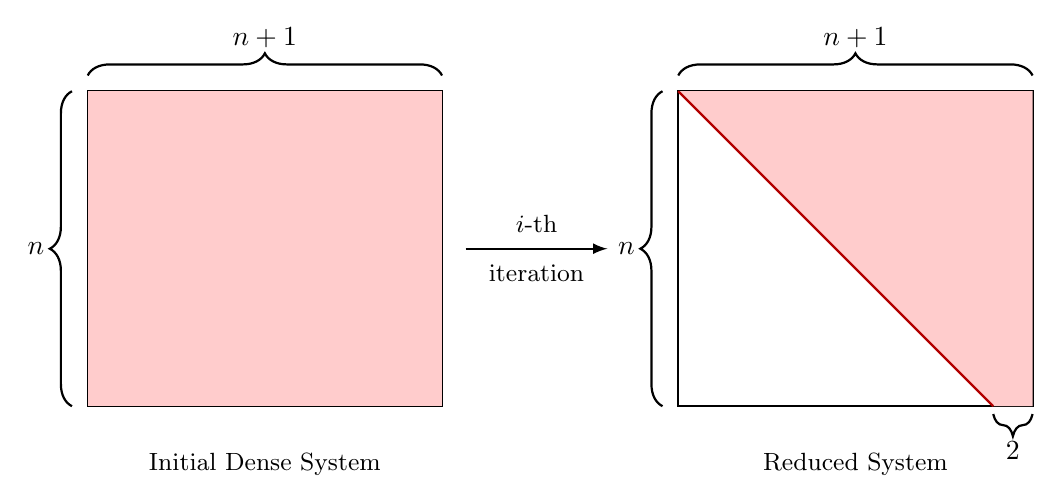
\begin{tikzpicture}[
    every node/.style={inner sep=0pt, outer sep=0pt},
    % Brace style
    curlybrace/.style={
        thick,
        decoration={brace, amplitude=8pt},
        decorate
    },
    % Matrix border style
    matrixbox/.style={
        draw=black,
        thick,
        fill=white
    }
]

% Global parameters (easy to scale)
\def\matH{4}       % Height of matrices (n)
\def\matW{4.5}     % Width of matrices (n+1)
\def\gap{3}        % Horizontal gap between matrices

% ================================
% 1. DENSE MATRIX (INITIAL SYSTEM)
% ================================
\begin{scope}[xshift=0cm]
    \draw[matrixbox] (0,0) rectangle (\matW,\matH);
    
    % Fully shaded
    \fill[fill=red!20] (0,0) rectangle (\matW,\matH);
    
    % Braces
    \draw[curlybrace] (-0.2,0) -- (-0.2,\matH) node[midway, left=10pt] {$n$};
    \draw[curlybrace] (0,\matH+0.2) -- (\matW,\matH+0.2) node[midway, above=10pt] {$n+1$};
    
    % Label below
    \node[anchor=north, font=\small] at (\matW/2, -0.6) {Initial Dense System};
\end{scope}

% ================================
% ARROW 1
% ================================
\draw[->, >=latex, thick] (\matW + 0.3, \matH/2) -- (\matW + \gap - 0.9, \matH/2)
    node[midway, above=6pt, font=\small, align=center] {$i$-th}
    node[midway, below=6pt, font=\small, align=center] {iteration};

% ================================
% 2. FINAL MATRIX (LINEAR RELATION)
% ================================
\begin{scope}[xshift=\matW cm + \gap cm]
    \draw[matrixbox] (0,0) rectangle (\matW,\matH);
    
    % Triangular shape
    \fill[fill=red!20] (0,\matH) -- (\matH,0) -- (\matW,0) -- (\matW,\matH) -- cycle;
    \draw[draw=red!70!black, thick] (0,\matH) -- (\matH,0);
    
    % Braces
    \draw[curlybrace] (-0.2,0) -- (-0.2,\matH) node[midway, left=10pt] {$n$};
    \draw[curlybrace] (0,\matH+0.2) -- (\matW,\matH+0.2) node[midway, above=10pt] {$n+1$};
    \draw[curlybrace] (\matW, -0.1) -- (\matH, -0.1) node[midway, below=10pt] {2};
    
    % Label below
    \node[anchor=north, font=\small] at (\matW/2, -0.6) {Reduced System};
\end{scope}

\end{tikzpicture}
    }
    \caption{Graphical overview of the REF step over 1 iteration.}\label{fig:overview}
\end{figure}

\subsection{Details of REF and Non-Linear Relations}

In the ideal scenario described, a single reduction of the coefficient matrix to Row Echelon Form (REF) immediately isolates a linear relation in the active variable $x_i$. However, in practice, a single REF computation does not strictly guarantee a degree 1 equation. It might happened that the last row gives us a relation of degree $d > 1$.

For instance, suppose the REF reduction yields a quadratic relation instead of a linear one:
\begin{equation}
    h_i^{(2)}(x_{i+1}, \dots, x_n) x_i^2 + h_i^{(1)}(x_{i+1}, \dots, x_n) x_i + h_i^{(0)}(x_{i+1}, \dots, x_n) = 0.
    \label{eq:quadratic_relation}
\end{equation}
To overcome this and force a linear relation, we employ an iterative degree-reduction. Using the relation obtained in Equation~\ref{eq:quadratic_relation}, we can express the leading term as a function of lower-degree terms:
\begin{equation*}
    h_i^{(2)}(x_{i+1}, \dots, x_n) x_i^2 = -\left( h_i^{(1)}(x_{i+1}, \dots, x_n) x_i + h_i^{(0)}(x_{i+1}, \dots, x_n) \right).
\end{equation*}

We then use this identity to systematically reduce the degree of $x_i$ in all other equations within the active system. To do this without introducing rational functions, we multiply the remaining polynomial equations by an appropriate power of the leading coefficient, ${(h_i^{(2)})}^k$. This homogenization step allows us to substitute every occurrence of ${(h_i^{(2)} x_i^2)}^k$ with the lower-degree equivalent ${\left( -h_i^{(1)} x_i - h_i^{(0)} \right)}^k$.

After applying this substitution across the entire system, the maximal degree of $x_i$ in the remaining equations is strictly reduced. We then reconstruct the univariate coefficient matrix for this newly updated system and perform the REF reduction again. 

Because the system is defined over the finite field $\Fq$ and augmented by the field equations $x_i^q - x_i = 0$, the roots are strictly bounded. Consequently, this iterative cycle of REF reduction and pseudo-division will decrease the minimum degree of the relations. By applying this process iteratively, the degree of the minimal relation will continually drop until a linear relation of the form showed in Equation~\ref{eq:linear_relation_i} is successfully extracted, allowing the main algorithm to proceed.

\begin{figure}[h!]
    \centering
    \resizebox{0.9\linewidth}{!}{
        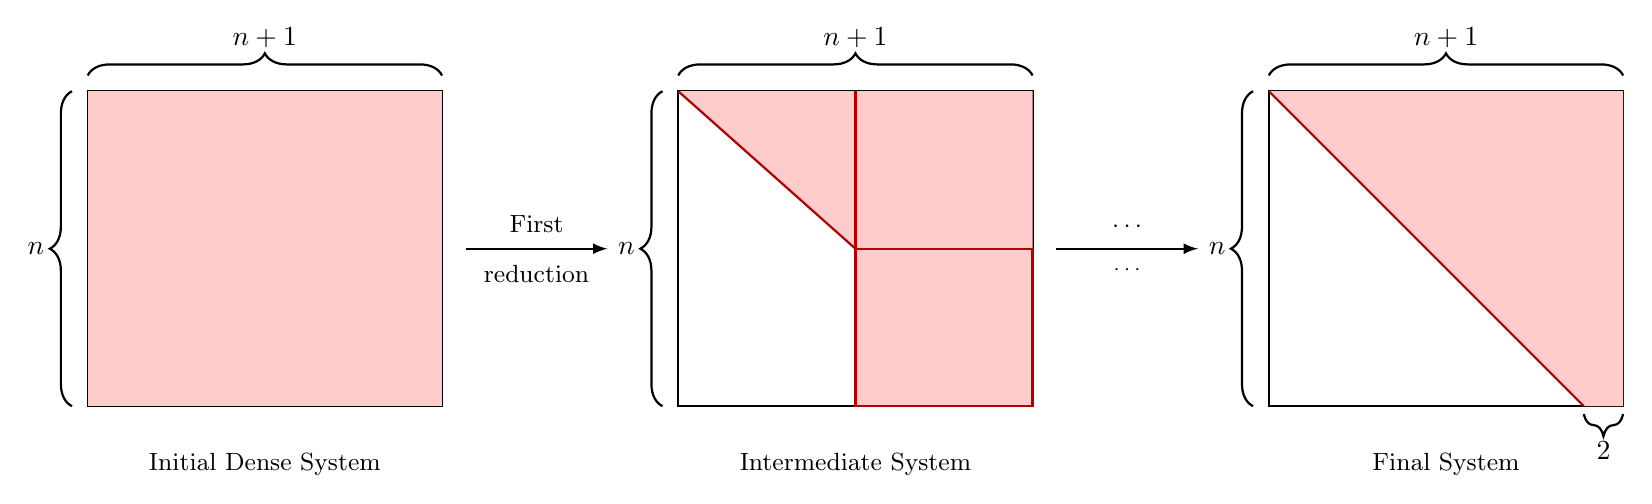
\begin{tikzpicture}[
    every node/.style={inner sep=0pt, outer sep=0pt},
    % Brace style
    curlybrace/.style={
        thick,
        decoration={brace, amplitude=8pt},
        decorate
    },
    % Matrix border style
    matrixbox/.style={
        draw=black,
        thick,
        fill=white
    }
]

% Global parameters (easy to scale)
\def\matH{4}       % Height of matrices (n)
\def\matW{4.5}     % Width of matrices (n+1)
\def\gap{3}        % Horizontal gap between matrices

% ================================
% 1. DENSE MATRIX (INITIAL SYSTEM)
% ================================
\begin{scope}[xshift=0cm]
    \draw[matrixbox] (0,0) rectangle (\matW,\matH);
    
    % Fully shaded
    \fill[fill=red!20] (0,0) rectangle (\matW,\matH);
    
    % Braces
    \draw[curlybrace] (-0.2,0) -- (-0.2,\matH) node[midway, left=10pt] {$n$};
    \draw[curlybrace] (0,\matH+0.2) -- (\matW,\matH+0.2) node[midway, above=10pt] {$n+1$};
    
    % Label below
    \node[anchor=north, font=\small] at (\matW/2, -0.6) {Initial Dense System};
\end{scope}

% ================================
% ARROW 1
% ================================
\draw[->, >=latex, thick] (\matW + 0.3, \matH/2) -- (\matW + \gap - 0.9, \matH/2)
    node[midway, above=6pt, font=\small, align=center] {First}
    node[midway, below=6pt, font=\small, align=center] {reduction};

% ================================
% 2. INTERMEDIATE MATRIX
% ================================
\begin{scope}[xshift=\matW cm + \gap cm]
    \draw[matrixbox] (0,0) rectangle (\matW,\matH);
    
    % Top shape
    \fill[fill=red!20] (0,\matH) -- (\matW/2,\matH/2) -- (\matW,\matH/2) -- (\matW,\matH) -- cycle;
    \draw[draw=red!70!black, thick] (0,\matH) -- (\matW/2,\matH/2); 
    \draw[draw=red!70!black, thick] (\matW/2,\matH/2) -- (\matW,\matH/2); 
    \draw[draw=red!70!black, thick] (\matW/2,\matH/2) -- (\matW/2,\matH); 
    
    % Lower square block
    \fill[fill=red!20] (\matW/2, 0) rectangle (\matW, \matH/2);
    \draw[draw=red!70!black, thick] (\matW/2, 0) rectangle (\matW, \matH/2);
    % Braces
    \draw[curlybrace] (-0.2,0) -- (-0.2,\matH) node[midway, left=10pt] {$n$};
    \draw[curlybrace] (0,\matH+0.2) -- (\matW,\matH+0.2) node[midway, above=10pt] {$n+1$};
    
    % Label below
    \node[anchor=north, font=\small] at (\matW/2, -0.6) {Intermediate System};
\end{scope}

% ================================
% ARROW 2
% ================================
\draw[->, >=latex, thick] (2*\matW + \gap + 0.3, \matH/2) -- (2*\matW + 2*\gap - 0.9, \matH/2)
    node[midway, above=6pt, font=\small, align=center] {$\cdots$}
    node[midway, below=6pt, font=\scriptsize, align=center] {$\cdots$};

% ================================
% 3. FINAL MATRIX (LINEAR RELATION)
% ================================
\begin{scope}[xshift=2*\matW cm + 2*\gap cm]
    \draw[matrixbox] (0,0) rectangle (\matW,\matH);
    
    % Triangular shape
    \fill[fill=red!20] (0,\matH) -- (\matH,0) -- (\matW,0) -- (\matW,\matH) -- cycle;
    \draw[draw=red!70!black, thick] (0,\matH) -- (\matH,0);
    
    % Braces
    \draw[curlybrace] (-0.2,0) -- (-0.2,\matH) node[midway, left=10pt] {$n$};
    \draw[curlybrace] (0,\matH+0.2) -- (\matW,\matH+0.2) node[midway, above=10pt] {$n+1$};
    \draw[curlybrace] (\matW, -0.1) -- (\matH, -0.1) node[midway, below=10pt] {2};

    
    % Label below
    \node[anchor=north, font=\small] at (\matW/2, -0.6) {Final System};
\end{scope}

\end{tikzpicture}
    }
    \caption{Graphical overview of a general reduction phase in a single iteration.}\label{fig:iteration}
\end{figure}